%------------------------------------------------------------------------------
% Template file for the submission of papers to IUCr journals in LaTeX2e
% using the iucr document class
% Copyright 1999-2013 International Union of Crystallography
% Version 1.6 (28 March 2013)
%------------------------------------------------------------------------------

\documentclass[preprint]{iucr}              % DO NOT DELETE THIS LINE
\usepackage{amssymb}
\usepackage[fleqn]{amsmath}
%\usepackage{bm}
\usepackage{graphicx}
\usepackage{tabularx}
\usepackage{booktabs}
%\usepackage{calligra}
\usepackage{array}
\DeclareMathAlphabet{\mathcalligra}{T1}{calligra}{m}{n}
\def\mathbi#1{\textbf{\em #1}}
\numberwithin{equation}{section}
%\DeclareMathSymbol{\Gamma}{\mathalpha}{letters}{"00}
%\DeclareMathSymbol{\Lambda}{\mathalpha}{letters}{"03}
%\DeclareMathSymbol{\Omega}{\mathalpha}{letters}{"0A}
%\DeclareMathAlphabet{\mathitbf}{OML}{cmm}{b}{it}
\hyphenation{Niggli}
\def\mathbi#1{\textbf{\em #1}}
%\numberwithin{equation}{section}
%\DeclareMathSymbol{\Gamma}{\mathalpha}{letters}{"00}
%\DeclareMathSymbol{\Lambda}{\mathalpha}{letters}{"03}
%\DeclareMathSymbol{\Omega}{\mathalpha}{letters}{"0A}
%\DeclareMathAlphabet{\mathitbf}{OML}{cmm}{b}{it}
\DeclareRobustCommand{\captionpar}{\par}
\usepackage{color}
\usepackage{ulem}
\usepackage{url}
\usepackage{yfonts}
\usepackage{relsize} 
\usepackage{wrapfig}
%\usepackage{xr-hyper}
%\usepackage[draft]{hyperref}
%\usepackage{bibentry}

\newcommand{\SVI}[0]{$\bf{S^{6}}$}
\newcommand{\GVI}[0]{$\bf{G^{6}}$}
\newcommand{\CIII}[0]{$\bf{C^{3}}$}
\newcommand{\DVII}[0]{$\bf{D^{7}}$}
\newcommand{\VVII}[0]{$\bf{V^{7}}$}

\newcommand{\vdotv}[2]{${{\bf #1 \cdot #2}}$}
\newcommand{\Imaginary}[0]{$ \textfrak{I} $}
\newcommand{\Real}[0]{$ \textfrak{R} $}
\newcommand{\Exchange}[0]{$\textfrak{X}$}

\newcommand{\nounderline}[3]{\!\!\!\!\!\!\!\!\!#1,&\!\!\!\!\!\!\!\!\!#2,&\!\!\!\!\!\!\!\!\!#3}
\newcommand{\underlineab}[3]{\!\!\!\!\!\!\!\!\!\!\!\!\!\!\!\!\!\!\!\!\!\!\!\!\Exchange{}(#1),&\!\!\!\!\!\!\!\!\!\!\!\!\!\!\!\!\!\!\!\!\!\!\!\!\Exchange{}(#2),&\!\!\!\!\!\!\!\!\!#3}
\newcommand{\underlineac}[3]{\!\!\!\!\!\!\!\!\!\!\!\!\!\!\!\!\!\!\!\!\!\!\!\!\Exchange{}(#1),&\!\!\!\!\!\!\!\!\!\!\!\!\!\!\!\!\!\!\!\!\!\!\!\!#2,&\!\!\!\!\!\!\!\!\!\Exchange{}(#3)}
\newcommand{\underlinebc}[3]{\!\!\!\!\!\!\!\!\!\!\!\!\!\!\!\!\!\!\!\!\!\!\!\!#1,&\!\!\!\!\!\!\!\!\!\Exchange{}(#2),&\!\!\!\!\!\!\!\!\!\!\!\!\!\!\!\!\!\!\!\!\!\!\!\!\Exchange{}(#3)}


\newcommand{\scalar}[1]{$#1$}

\newcommand{\scalarsub}[2]{$#1_#2$}

%-------------------------------------------------------------------------
% Information about journal to which submitted
%-------------------------------------------------------------------------
\journalcode{A}              % Indicate the journal to which submitted
%   A - Acta Crystallographica Section A
%   B - Acta Crystallographica Section B
%   C - Acta Crystallographica Section C
%   D - Acta Crystallographica Section D
%   E - Acta Crystallographica Section E
%   F - Acta Crystallographica Section F
%   J - Journal of Applied Crystallography
%   M - IUCrJ
%   S - Journal of Synchrotron Radiation
\makeatletter
\font\dummyft@=dummy \relax
\makeatother


\begin{document}                  % DO NOT DELETE THIS LINE

	\raggedbottom
	\setlength{\parskip}{0pt}
	{\LARGE \emph{\today}} \\
%	\title{Measuring Lattices}
%	%\title{Note on the transformation of three-space basis vectors to  corresponding matrix for Delaunay scalars}
%	\shorttitle{Measuring Lattices}
		
	
	\cauthor[a]{Lawrence C.}{Andrews}{larry6640995@gmail.com}{}
	\author[b]{Herbert J.}{Bernstein}
	
	\aff[a]{Ronin Institute, 9515 NE 137th St, Kirkland, WA, 98034-1820 \country{USA}}
	\aff[b]{Ronin Institute, c/o NSLS-II, Brookhaven National Laboratory, Upton, NY, 11973-5000 \country{USA}}
	
	
	% PDB and NDB reference codes for structures referenced in the article and
	% deposited with the Protein Data Bank and Nucleic Acids Database (Acta
	% Crystallographica Section D). Repeat for each separate structure e.g
	% \PDBref[dethiobiotin synthetase]{1byi} \NDBref[d(G$_4$CGC$_4$)]{ad0002}
	
	%\PDBref[optional name]{refcode}
	%\NDBref[optional name]{refcode}
	
	\maketitle                        % DO NOT DELETE THIS LINE
	\newcommand{\si}[0]{$s_1$}
	\newcommand{\sii}[0]{$s_2$}
	\newcommand{\siii}[0]{$s_3$}
	\newcommand{\siv}[0]{$s_4$}
	\newcommand{\sv}[0]{$s_5$}
	\newcommand{\svi}[0]{$s_6$}
	\newcommand{\Svec} [0] {\{\si, \sii, \siii, \siv, \sv, \svi \}}
	\newcommand{\SvecA} [0] {\{-\si, -\si+\sii, \si+\siii, \si+\sv, \si+\siv, \si+\svi \}}
	
	\newcommand{\OPES}[0]{$E^3toS^6$}
	\newcommand{\OPESS}[0]{$$E^3toS^6$$}
	\newcommand{\MSVI}[0]{$M_{S^{6}}$}
	\newcommand{\MEIII}[0]{$M_{E^{3}}$}
	\newcommand{\Plus}[0]{$\textfrak{P}$}	
	\newcommand{\Minus}[0]{$\textfrak{M}$}
	
	\newcommand{\ci}[0]{$c_1$}
	\newcommand{\cii}[0]{$c_2$}
	\newcommand{\ciii}[0]{$c_3$}
	
	
	
	%-------------------------------------------------------------------------
	% The main body of the paper
	%-------------------------------------------------------------------------
	% Now enter the text of the document in multiple \section's, \subsection's
	% and \subsubsection's as required.
	

	\section{History}
	
	Human fascination with crystals has a long history. 105,000 years ago,
	someone had a collection of calcite crystals 
	(Iceland spar) \cite{wilkins2021innovative}. 
	Theophrastus (ca. 372-287 B.C.), a student of Plato and successor to Aristotle, wrote the first known treatise on gems (``On Stones'')  \cite{enwiki:1114534722}.
	
	Figure \ref{timeline} notes a few key events in cataloging 
	crystal properties. We start with \cite{Kepler1611} (translated in \cite{kepler1966}) and Steno  (see \cite{authier2013early}) who
	conjectured on the structures of crystals.  \cite{hauy1800addition} created the first catalog of minerals.
	
	\begin{figure}
		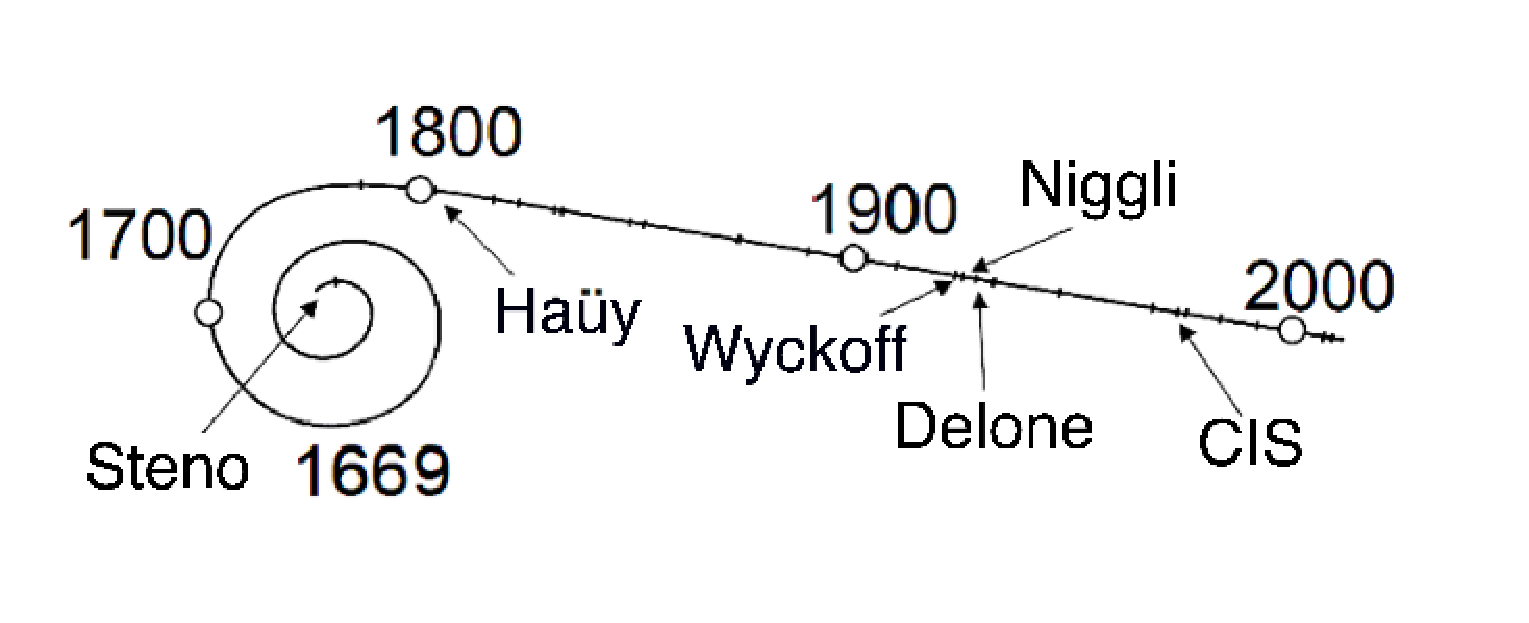
\includegraphics[width=\textwidth]{TimeLine_rev}
		\label{timeline}
		\caption{Some key dates in the history of modern crystallography}
	\end{figure}
	
	
	\section{References to Sources for Information about the Calculations}
\begin{itemize}
	\item 	\emph{No operation:} simply check the input for errors
	\item 	\emph{generate four C6 test cells}
	\item 	\emph{compute Selling-reduced primitive cells:} Delone/Delaunay/Selling reduction \\
	\cite{Delaunay1932}\\
	\cite{Delone1975}\\
	\cite{Andrews2019a}
	\item 	\emph{compute NCDist and CS6Dist distances}\\
	\cite{Andrews2014}\\
	\cite{Andrews2019b}
	\item \emph{	apply Lattice Matching algorithm to listed cells}\\
	\cite{Mighell2002}\\
	\cite{andrews2021approximate}
	\item 	\emph{compute Niggli-reduced primitive cells}\\
	\cite{Niggli1928}
	\cite{Gruber1973}
	\item 	\emph{compute path between pairs of cells}\\
	\cite{andrews2023follower}
	\item 	\emph{compute perturbed versions of input cells}\\
	\cite{andrews2022generating}
	\item 	\emph{apply S6 reflections to input cells}\\
	\cite{Andrews2019b}
	\item 	\emph{apply Sella algorithm}\\
	\cite{andrews2023sella}
	\item 	\emph{compute Bravais tetrahedron (B4)}\\
	\cite{Delone1975}
	\item 	\emph{compute Selling-reduced complex cell presentation (C3)}\\
	\cite{Andrews2019b}
	\item 	\emph{compute side-angle cells (a, b, c, $\alpha$, $\beta$, $\gamma$)}
	\item 	\emph{compute raw Dirichlet cells (DC13)}\\
	\cite{Bernstein2023}
	\item 	\emph{computed sorted Dirichlet cells (DC)}\\
	\cite{Bernstein2023}
	\item 	\emph{compute Niggli-reduced cells (G6)}\\
	\cite{Andrews2014}
	\item 	\emph{compute Selling-reduced cells (S6)}\\
	\cite{Andrews2019b}
	\item 	\emph{compute unsorted Dirichlet cells (dc7unsrt)}\\
	\cite{Andrews2019b}
	\item 	\emph{compute volumes of listed cells}
\end{itemize}	

%			\ack{{\bf Funding information}}      
%			
%			Funding for this research was provided in part by:  
%			US Department of Energy Offices of Biological and 
%			Environmental Research and of Basic Energy Sciences 
%			(grant No. DE-AC02-98CH10886; grant No. E-SC0012704); 
%			U.S. National Institutes of Health (grant No. P41RR012408; 
%			grant No. P41GM103473; grant No. P41GM111244; 
%			grant No. R01GM117126,
%			grant No. 1R21GM129570); Dectris, Ltd.
			
			
			\bibliography{Reduced}
			
			\bibliographystyle{iucr}
			
			
			
			%-------------------------------------------------------------------------
			% TABLES AND FIGURES SHOULD BE INSERTED AFTER THE MAIN BODY OF THE TEXT
			%-------------------------------------------------------------------------
			
			% Simple tables should use the tabular environment according to this
			% model
			
			% Postscript figures can be included with multiple figure blocks
			
			
			
		\end{document}                    % DO NOT DELETE THIS LINE
		%%%%%%%%%%%%%%%%%%%%%%%%%%%%%%%%%%%%%%%%%%%%%%%%%%%%%%%%%%%%%%%%%%%%%%%%%%%%%%
